\DiaryEntry{Least Squares}{2015-06-26}{Maths}


Derivation of the least-squares expression: Given the system matrix \(\mathbf{A}\) and the observation \(\mathbf{y}\), we seek the \(\mathbf{\hat{x}}\) so that the error \(\mathbf{r} = \mathbf{y} - \mathbf{A} \mathbf{x}\) is minimized.

%\pagebreak

\begin{figure}[htb!]
\centering
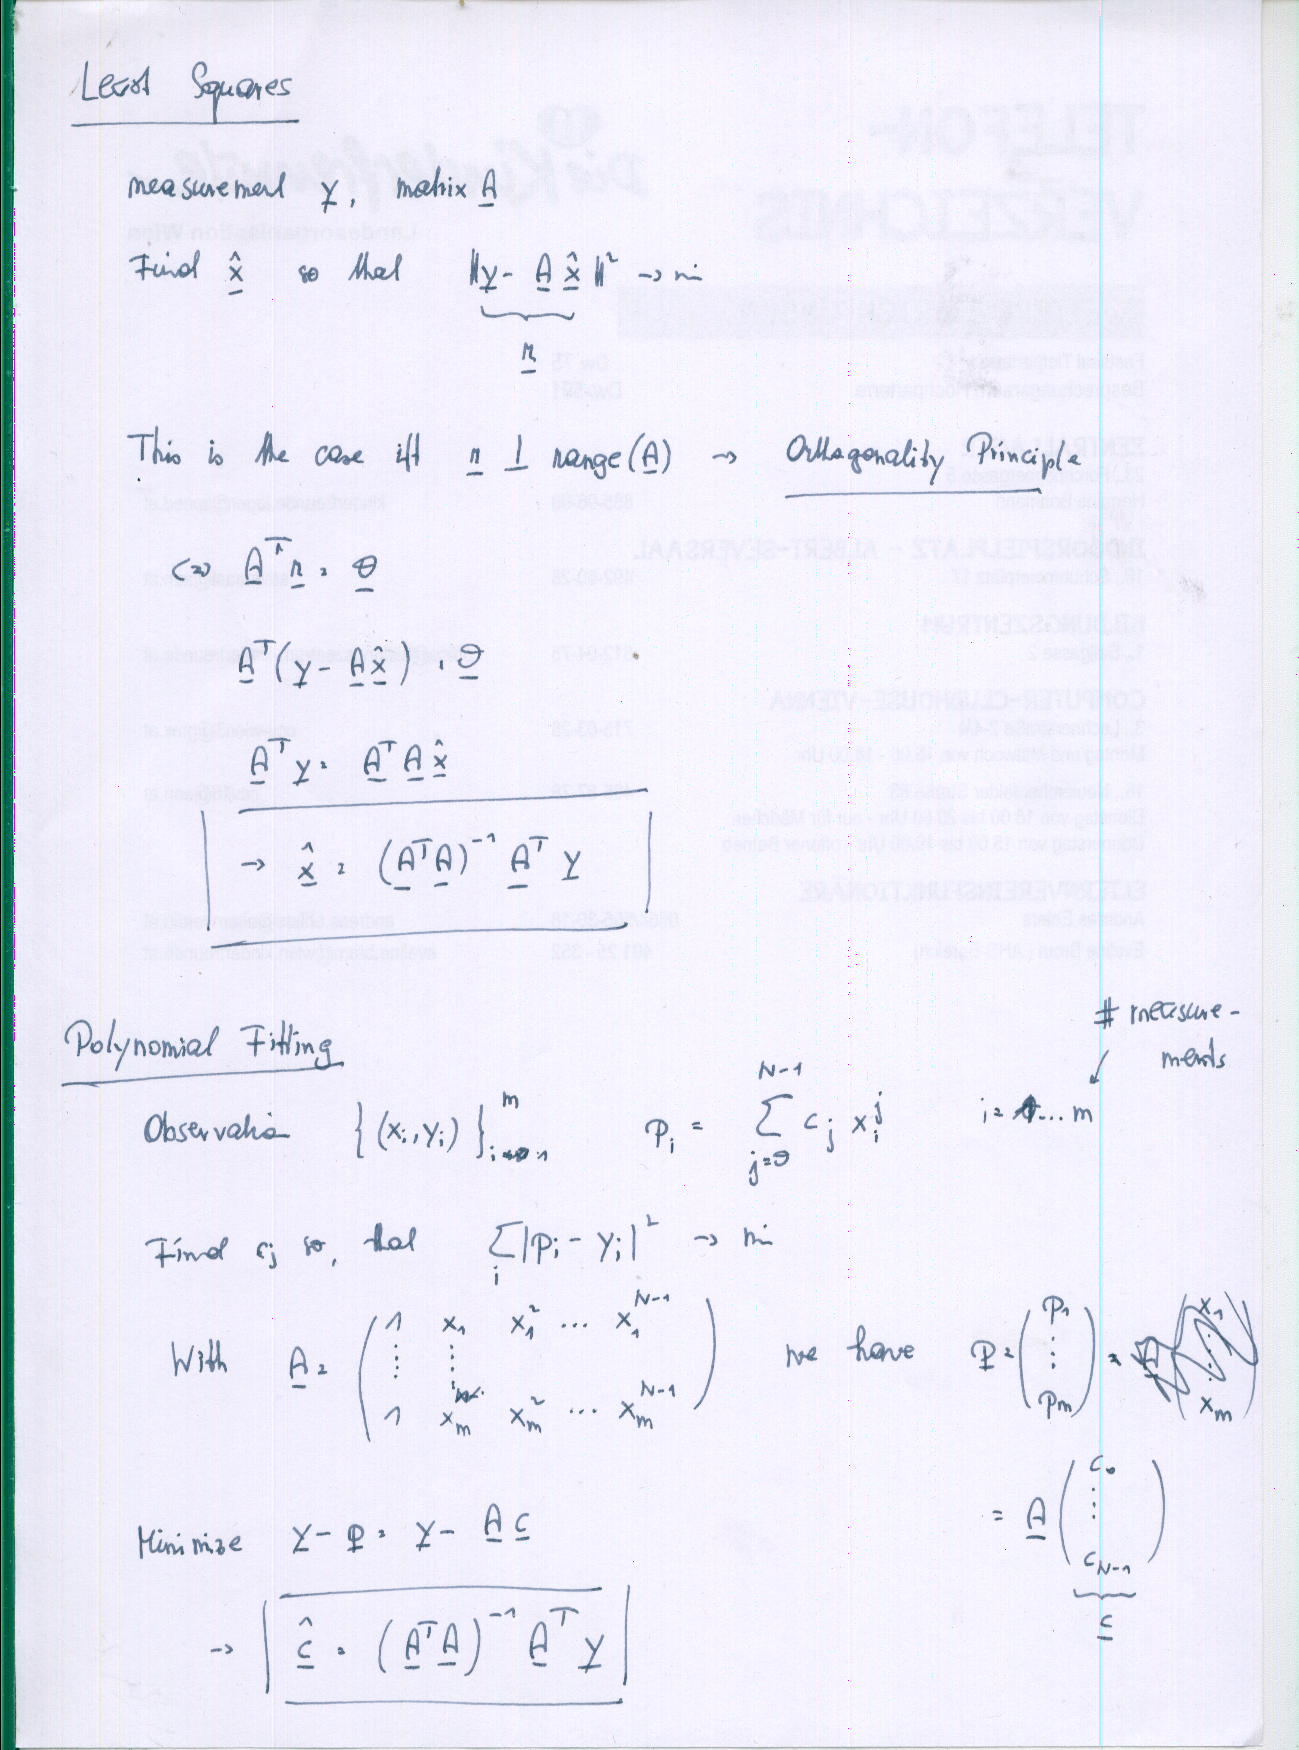
\includegraphics[scale=0.5]{images/least_squares.png}
\caption{Derivation}
\end{figure}

Seen another way, the result \(\mathbf{\hat{x}} = (\mathbf{A}^T \mathbf{A})^{-1} \mathbf{A}^T \mathbf{y}\) is the projection of \(\mathbf{y}\) onto the vector space defined by the columns of \(\mathbf{A}\).

\subsection{Least Squares Example (Julia)}

We consider \(\mathbb{R}^3\) and want to project onto the x-y plane; first we choose the matrix \(\mathbf{A} = [\mathbf{e_1} \mathbf{e_2}]\)

\begin{verbatim}
A=[1 0;0 1;0 0]
inv(A'*A)*A'

2x3 Array{Float64,2}:
1.0  0.0  0.0
0.0  1.0  0.0
\end{verbatim}

The least squares matrix considers only the first two components of any vector it is applied onto =\textgreater{} projection onto x-y plane.

Similarly, nothing (much) changes, if we choose different vectors \(\mathbf{u_1}, \mathbf{u_2}\) for \(\mathbf{A} = [\mathbf{u_1} \mathbf{u_2}]\), as long as they are part of the x-y plane:

\begin{verbatim}
A=[sqrt(2)/2 -sqrt(2)/2;sqrt(2)/2 sqrt(2)/2;0 0]

3x2 Array{Float64,2}:
0.707107  -0.707107
0.707107   0.707107
0.0        0.0     

inv(A'*A)*A'

2x3 Array{Float64,2}:
0.707107  0.707107  0.0
-0.707107  0.707107  0.0
\end{verbatim}

\subsection{Least Squares Polynomial Fitting Example (Julia)}

\subsubsection{No Noise}

We consider \(x_i={-2,-1.2,-0.4,0.4,1.2,2}\) and $y_i=x_i^3$. We least-squares fit three polynoms onto the point set \({x_i,y_i}\) with degree \(N=1\) (a straight line); \(N=3\) (a polynom of the same order as the ``model''), and \(N=6\); i.e. a polynomial with a higher order.

\begin{verbatim}
using Winston

N = 6
srand(1234)

x = linspace(-2,2,N)
y = x.^3

yobs = y

A1 = [x.^0 x.^1]
A3 = [x.^0 x.^1 x.^2 x.^3]
A5 = [x.^0 x.^1 x.^2 x.^3 x.^4 x.^5]


c_hat_1 = inv(A1'*A1)*A1'*yobs
c_hat_3 = inv(A3'*A3)*A3'*yobs
c_hat_5 = inv(A5'*A5)*A5'*yobs

plot(x,yobs,"-rx", x,A1*c_hat_1,"ob", x,A3*c_hat_3,"og", x,A5*c_hat_5,"oy")
savefig("ls_polyfit.pdf")
\end{verbatim}

The following plot shows the results for these different degrees. The observed data is shown in red with circles. The polynomial with $N=1$ (blue circles) gives a bad fit; both $N=3$ (green circles) and $N = 6$ (yellow pluses) yield a pefect match.

\begin{figure}[htb!]
\centering
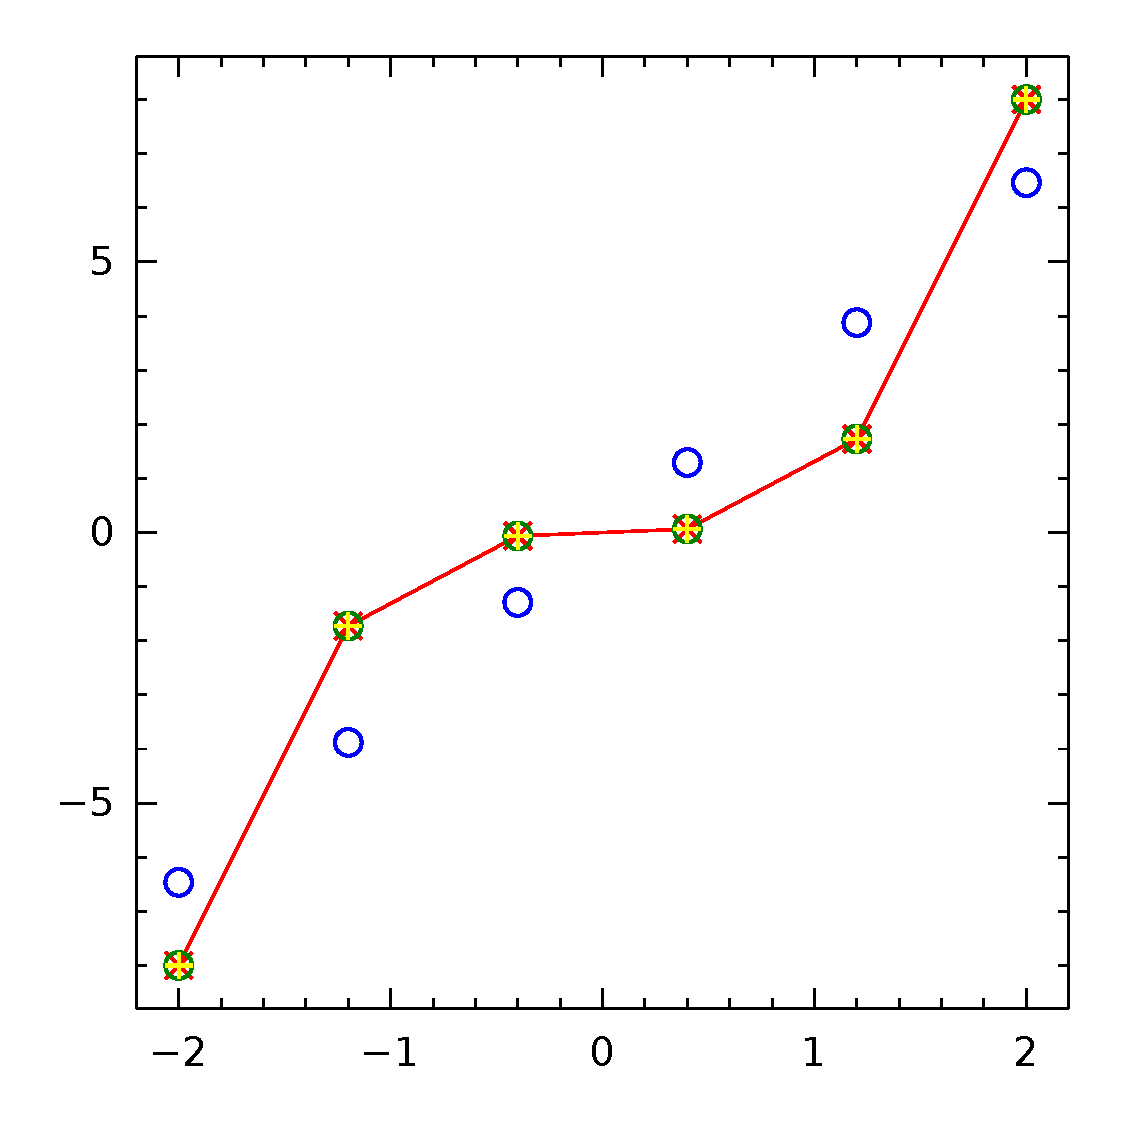
\includegraphics[scale=0.5]{images/ls_polyfit_no_noise.pdf}
\caption{Approximation of noise-free observation with polynomials of degree 1, degree 3, and degree 6, respectively.}
\end{figure}

The coefficient values are as follows

\begin{verbatim}
c_hat_3
4-element Array{Float64,1}:
 0.0       
 1.9984e-15
 0.0       
 1.0

c_hat_5
6-element Array{Float64,1}:
 0.0        
 4.59077e-14
 1.11022e-16
 1.0        
 0.0        
 2.89768e-14

\end{verbatim}

That is, they perfectly match the polynomial $x^3$.


\subsubsection{Measurement with Noise}

Things become different, when the observations are noisy; i.e. $y_i=x_i^3 + w_i$ with the $w_i$ some random Gaussian noise having variance $1$.

The plot below shows the results in this case. It can be seen that the polynomial $N=3$ is now an imperfect match while the polynomial with $N=6$ still has a perfect match: A polynomial of degree $6$ can perfectly match a sequence of $6$ datapoints.


\begin{figure}[htb!]
\centering
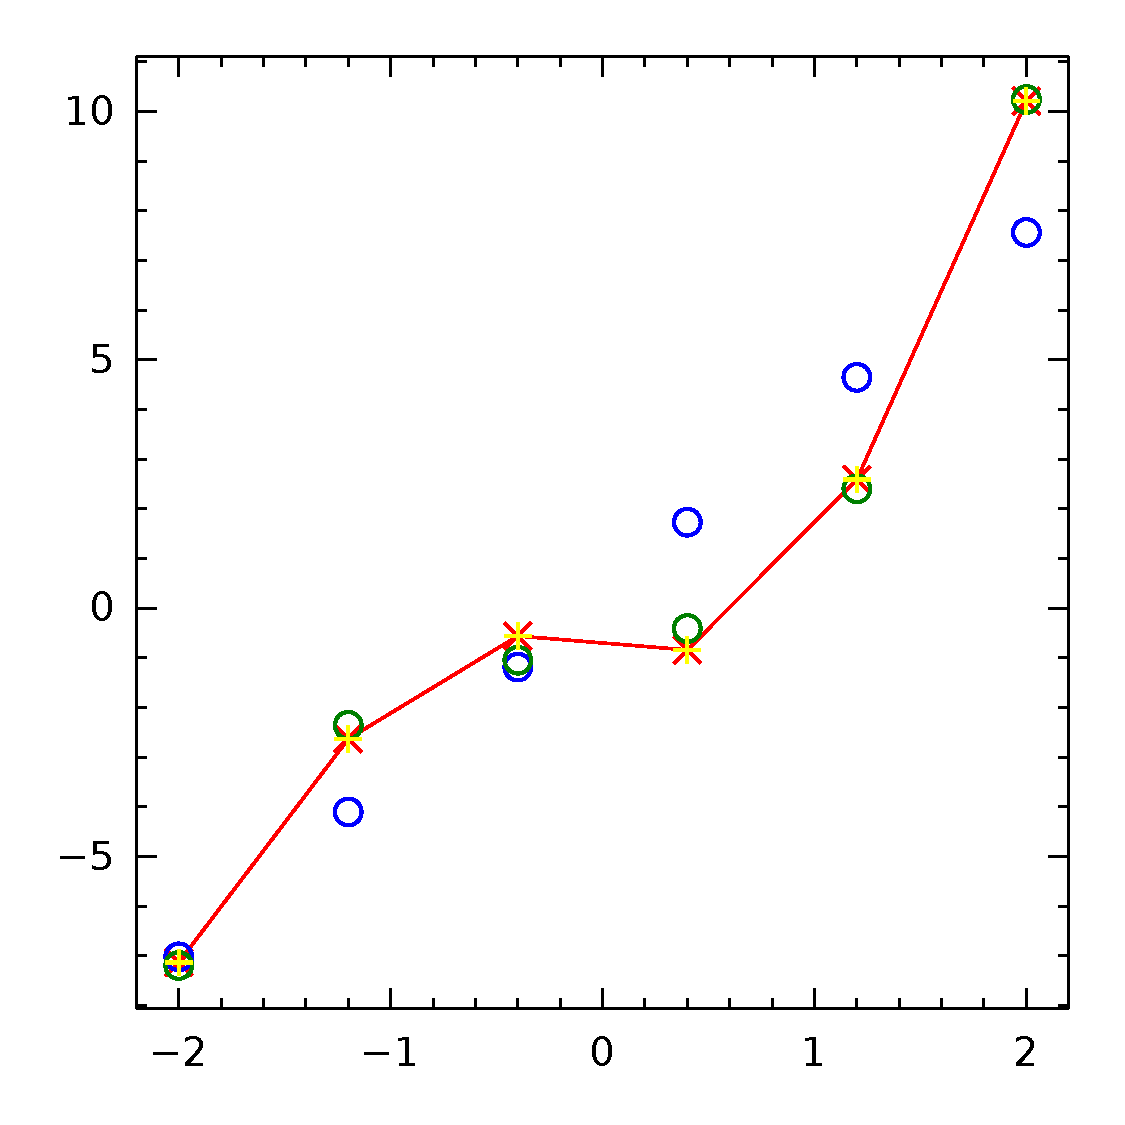
\includegraphics[scale=0.5]{images/ls_polyfit_with_noise.pdf}
\caption{Approximation of noise observation with polynomials of degree 1, degree 3, and degree 6, respectively.}
\end{figure}
